\chapter{Metodologia}
\label{cap:metodologia}

Este trabalho caracteriza-se como uma pesquisa aplicada, de abordagem quantitativa, com uso de simulação computacional. A pesquisa é aplicada porque busca analisar um problema prático relacionado ao uso de redes LoRaWAN no monitoramento de ovinos em ambiente rural, considerando cenários próximos à realidade da ovinocultura no Sertão Central. Assim, o estudo não tem como finalidade propor um novo protocolo de comunicação, um novo algoritmo de adaptação de taxa ou um novo dispositivo físico, mas avaliar o comportamento de uma rede LoRaWAN simulada diante da variação na quantidade de nós sensores.

A abordagem quantitativa deve-se ao fato de que a análise será realizada a partir de dados numéricos obtidos nas simulações. Esses dados serão representados por métricas de desempenho da rede, como taxa de entrega de pacotes, Packet Delivery Ratio (PDR), perdas de pacotes e consumo energético estimado dos dispositivos. A partir dessas métricas, será possível comparar os resultados entre diferentes configurações de rede e entre os cenários de confinamento e pastagem.

A simulação computacional será utilizada como meio para representar uma rede de monitoramento formada por dispositivos sensores instalados nos animais, um gateway e a infraestrutura de comunicação LoRaWAN. Essa abordagem permite avaliar previamente o comportamento da rede em diferentes condições, sem a necessidade de implantação física de uma grande quantidade de dispositivos em campo.

\section{Procedimentos Metodológicos}
\label{sec:procedimentos-metodologicos}

A execução deste trabalho será organizada em etapas sequenciais, de modo que cada etapa contribua para o atendimento dos objetivos específicos definidos. Inicialmente, serão levantados e selecionados os parâmetros necessários para a simulação. Em seguida, serão modelados os cenários de confinamento e pastagem, configurada a rede LoRaWAN, executadas as simulações, coletadas as métricas de desempenho e realizada a análise comparativa dos resultados.

Para a realização das simulações, será utilizado o NS-3, ferramenta adotada neste trabalho para configurar a rede LoRaWAN, representar os cenários propostos e coletar as métricas de desempenho da comunicação.

A Figura~\ref{fig:fluxograma-metodologia} apresenta o fluxograma das etapas metodológicas previstas para o desenvolvimento deste trabalho. A representação visual
tem como finalidade organizar a sequência de atividades que serão realizadas, desde a definição dos parâmetros de simulação até a análise dos resultados obtidos.

\begin{figure}[h!]
    \captionsetup{width=16cm}
    \Caption{\label{fig:fluxograma-metodologia} Fluxograma das etapas metodológicas}
    \UFCfig{}{
        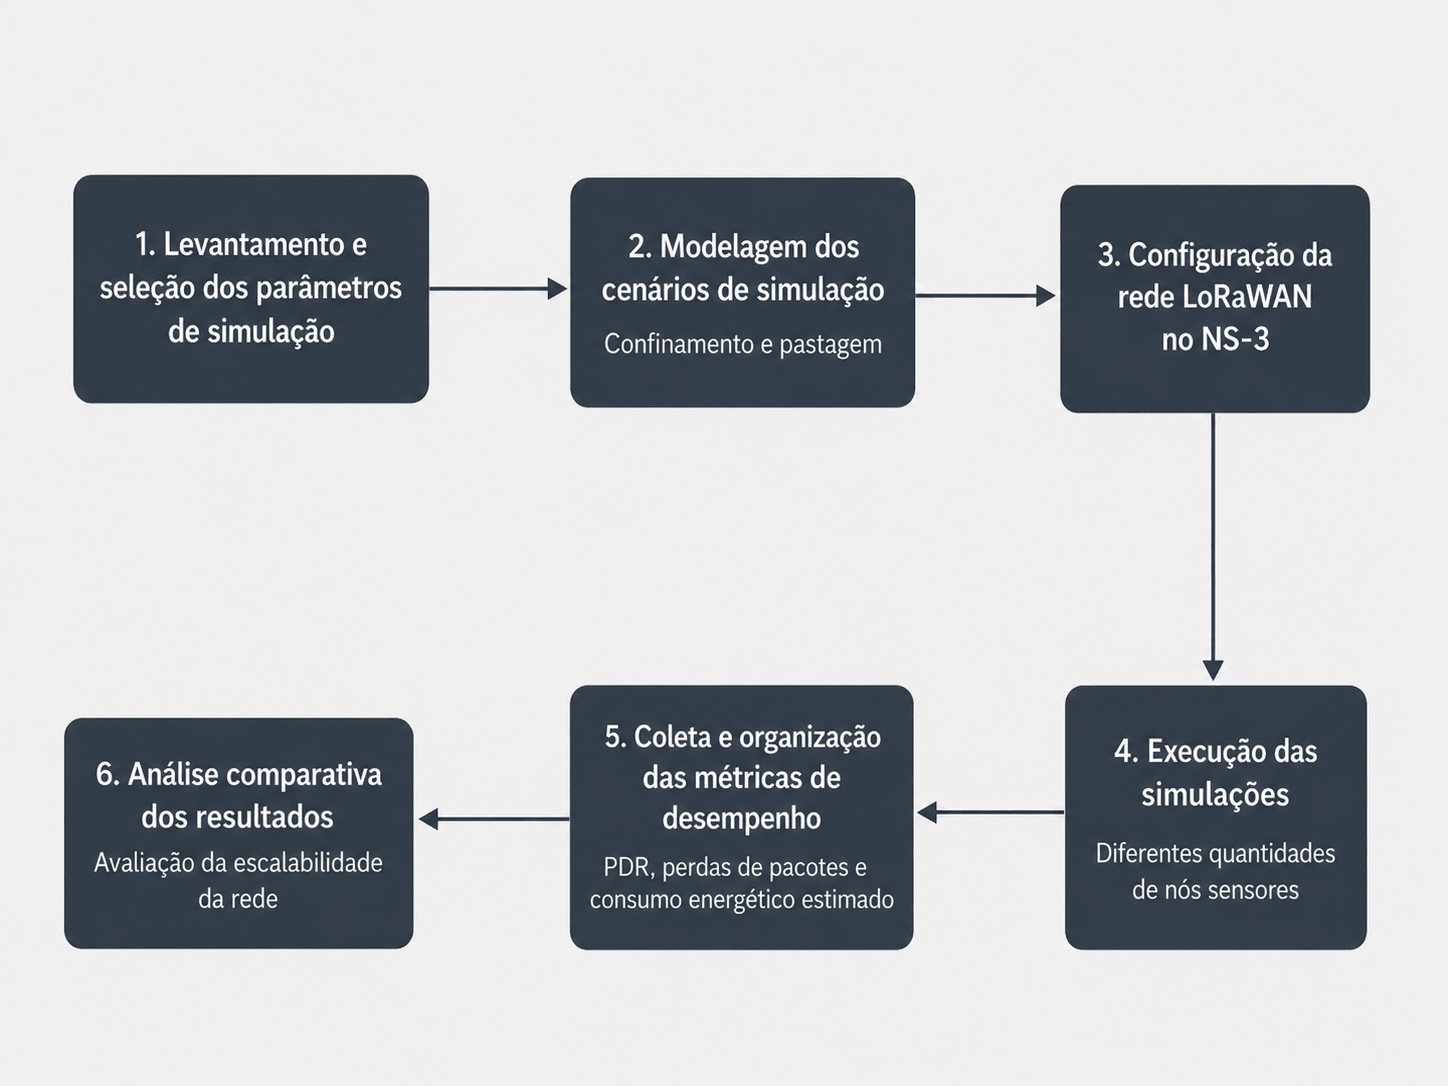
\includegraphics[width=16cm]{figuras/fluxograma-metodologia.png}
    }{
        \Fonte{Elaborado pelo autor com auxílio de ferramenta de inteligência artificial generativa (2026).}
    }
\end{figure}

Conforme apresentado na Figura~\ref{fig:fluxograma-metodologia}, a metodologia inicia-se com o levantamento e a seleção dos parâmetros de simulação, etapa necessária para definir as informações que serão representadas no ambiente computacional. Em seguida, são modelados os cenários de confinamento e pastagem e configurada a rede LoRaWAN no NS-3. Após essa configuração, serão executadas simulações com diferentes
quantidades de nós sensores, possibilitando a coleta das métricas de desempenho e a posterior comparação dos resultados. Dessa forma, as etapas metodológicas foram
organizadas para permitir a avaliação da escalabilidade da rede no contexto do monitoramento de ovinos.

\subsection{Levantamento e seleção dos parâmetros de simulação}
\label{subsec:parametros-simulacao}

A primeira etapa consistirá no levantamento dos parâmetros necessários para a simulação da rede LoRaWAN aplicada ao monitoramento de ovinos. Serão considerados aspectos como quantidade de nós sensores, intervalo de transmissão dos dados, área de cobertura, parâmetros de comunicação, características dos cenários analisados e métricas de avaliação de desempenho.

Após o levantamento inicial, serão selecionados os parâmetros que poderão ser representados no ambiente de simulação. Essa seleção levará em conta os recursos disponíveis na ferramenta adotada, as informações obtidas nos trabalhos relacionados e o perfil de monitoramento utilizado como referência. O protótipo desenvolvido por \citeonline{araujo2024} será utilizado como base prática para definir o tipo de dado monitorado e o envio periódico das informações pelos dispositivos sensores.

\subsection{Modelagem dos cenários de simulação}
\label{subsec:modelagem-cenarios}

A segunda etapa consistirá na modelagem dos cenários de confinamento e pastagem. Em ambos os cenários, os ovinos serão representados como nós sensores responsáveis pelo envio periódico de dados de monitoramento.

No cenário de confinamento, os nós sensores serão distribuídos em uma área menor, representando uma situação de maior concentração dos animais. No cenário de pastagem, os nós serão distribuídos em uma área mais ampla, representando maior dispersão espacial dos ovinos. A definição desses cenários buscará manter coerência com as características de manejo discutidas na fundamentação teórica.

\subsection{Configuração da rede LoRaWAN no NS-3}
\label{subsec:configuracao-rede}

A terceira etapa consistirá na configuração da rede LoRaWAN no NS-3. A rede será composta por nós sensores, responsáveis pelo envio periódico dos dados, e por um gateway, responsável pelo recebimento das transmissões.

Nessa etapa, serão configurados os parâmetros de comunicação da rede, a disposição dos dispositivos nos cenários, o intervalo de envio das mensagens e as condições necessárias para a execução das simulações. A quantidade de nós sensores será variada gradualmente, permitindo observar o comportamento da rede conforme aumenta o número de dispositivos transmitindo dados.

\subsection{Execução das simulações}
\label{subsec:execucao-simulacoes}

A quarta etapa consistirá na execução das simulações para cada cenário definido. As simulações serão realizadas considerando diferentes quantidades de nós sensores, de forma a avaliar o impacto do aumento no número de dispositivos sobre o desempenho da comunicação.

Cada configuração será executada no ambiente de simulação, mantendo-se o registro dos resultados obtidos para posterior comparação. Essa etapa permitirá observar o comportamento da rede em situações de maior concentração dos nós, como no confinamento, e em situações de maior dispersão espacial, como na pastagem.

\subsection{Coleta e organização das métricas}
\label{subsec:coleta-metricas}

A quinta etapa consistirá na coleta e organização das métricas de desempenho obtidas nas simulações. Entre as métricas previstas estão a taxa de entrega de pacotes, Packet Delivery Ratio (PDR), as perdas de pacotes e o consumo energético estimado dos dispositivos.

Os dados coletados serão organizados em tabelas, gráficos ou outros recursos que facilitem a comparação entre as configurações simuladas. Essa organização permitirá observar como a variação na quantidade de nós sensores influencia o desempenho da rede em cada cenário.

\subsection{Análise comparativa dos resultados}
\label{subsec:analise-resultados}

Por fim, será realizada a análise comparativa dos resultados obtidos. A análise buscará identificar como o aumento da quantidade de nós sensores influencia o desempenho da rede LoRaWAN e quais diferenças podem ser observadas entre os cenários de confinamento e pastagem.

A partir dessa comparação, será possível avaliar a escalabilidade da rede no contexto proposto, considerando as métricas definidas e as limitações do ambiente simulado.